%
% This is a borrowed LaTeX template file for lecture notes for CS267,
% Applications of Parallel Computing, UCBerkeley EECS Department.
% Now being used for CMU's 10725 Fall 2012 Optimization course
% taught by Geoff Gordon and Ryan Tibshirani.  When preparing 
% LaTeX notes for this class, please use this template.
%
% To familiarize yourself with this template, the body contains
% some examples of its use.  Look them over.  Then you can
% run LaTeX on this file.  After you have LaTeXed this file then
% you can look over the result either by printing it out with
% dvips or using xdvi. "pdflatex template.tex" should also work.
%

\documentclass[twoside]{article}
\setlength{\oddsidemargin}{0.25 in}
\setlength{\evensidemargin}{-0.25 in}
\setlength{\topmargin}{-0.6 in}
\setlength{\textwidth}{6.5 in}
\setlength{\textheight}{8.5 in}
\setlength{\headsep}{0.75 in}
\setlength{\parindent}{0 in}
\setlength{\parskip}{0.1 in}

%
% ADD PACKAGES here:
%

\usepackage{amsmath,amsfonts,graphicx}

%
% The following commands set up the lecnum (lecture number)
% counter and make various numbering schemes work relative
% to the lecture number.
%
\newcounter{lecnum}
\renewcommand{\thepage}{\thelecnum-\arabic{page}}
\renewcommand{\thesection}{\thelecnum.\arabic{section}}
\renewcommand{\theequation}{\thelecnum.\arabic{equation}}
\renewcommand{\thefigure}{\thelecnum.\arabic{figure}}
\renewcommand{\thetable}{\thelecnum.\arabic{table}}

%
% The following macro is used to generate the header.
%
\newcommand{\lecture}[4]{
   \pagestyle{myheadings}
   \thispagestyle{plain}
   \newpage
   \setcounter{lecnum}{#1}
   \setcounter{page}{1}
   \noindent
   \begin{center}
   \framebox{
      \vbox{\vspace{2mm}
    \hbox to 6.28in { {\bf 10-725: Optimization
	\hfill Fall 2012} }
       \vspace{4mm}
       \hbox to 6.28in { {\Large \hfill Lecture #1: #2  \hfill} }
       \vspace{2mm}
       \hbox to 6.28in { {\it Lecturer: #3 \hfill Scribes: #4} }
      \vspace{2mm}}
   }
   \end{center}
   \markboth{Lecture #1: #2}{Lecture #1: #2}

   {\bf Note}: {\it LaTeX template courtesy of UC Berkeley EECS dept.}

   {\bf Disclaimer}: {\it These notes have not been subjected to the
   usual scrutiny reserved for formal publications.  They may be distributed
   outside this class only with the permission of the Instructor.}
   \vspace*{4mm}
}
%
% Convention for citations is authors' initials followed by the year.
% For example, to cite a paper by Leighton and Maggs you would type
% \cite{LM89}, and to cite a paper by Strassen you would type \cite{S69}.
% (To avoid bibliography problems, for now we redefine the \cite command.)
% Also commands that create a suitable format for the reference list.
\renewcommand{\cite}[1]{[#1]}
\def\beginrefs{\begin{list}%
        {[\arabic{equation}]}{\usecounter{equation}
         \setlength{\leftmargin}{2.0truecm}\setlength{\labelsep}{0.4truecm}%
         \setlength{\labelwidth}{1.6truecm}}}
\def\endrefs{\end{list}}
\def\bibentry#1{\item[\hbox{[#1]}]}

%Use this command for a figure; it puts a figure in wherever you want it.
%usage: \fig{NUMBER}{SPACE-IN-INCHES}{CAPTION}
\newcommand{\fig}[3]{
			\vspace{#2}
			\begin{center}
			Figure \thelecnum.#1:~#3
			\end{center}
	}
% Use these for theorems, lemmas, proofs, etc.
\newtheorem{theorem}{Theorem}[lecnum]
\newtheorem{lemma}[theorem]{Lemma}
\newtheorem{proposition}[theorem]{Proposition}
\newtheorem{claim}[theorem]{Claim}
\newtheorem{corollary}[theorem]{Corollary}
\newtheorem{definition}[theorem]{Definition}
\newenvironment{proof}{{\bf Proof:}}{\hfill\rule{2mm}{2mm}}

% **** IF YOU WANT TO DEFINE ADDITIONAL MACROS FOR YOURSELF, PUT THEM HERE:

\newcommand\E{\mathbb{E}}

\begin{document}
%FILL IN THE RIGHT INFO.
%\lecture{**LECTURE-NUMBER**}{**DATE**}{**LECTURER**}{**SCRIBE**}
\lecture{1}{September 25}{Geoff Gordon/Ryan Tibshirani}{Subhodeep Moitra}
%\footnotetext{These notes are partially based on those of Nigel Mansell.}

% **** YOUR NOTES GO HERE:

% Some general latex examples and examples making use of the
% macros follow.  
%**** IN GENERAL, BE BRIEF. LONG SCRIBE NOTES, NO MATTER HOW WELL WRITTEN,
%**** ARE NEVER READ BY ANYBODY.


\section{Accelerated Backtracking Line Search} % Don't be this informal in your notes!
In the proof for accelerated general gradient descent we saw an $O(1/k^2)$ convergence rate which optimal. Gradient descent on the other hand has a $O(1/k)$ convergence rate. The proofs for these convergence rates are very different and are made under different assumptions. There are a number of different accelerated backtracking schemes and these are made under different criteria for the same reason. We will examine one of the simpler schemes. 


The assumptions that this scheme needs to make are : 
\begin{itemize}
\item Lipschitz Gradient condition
\[ 
	g(x^+) \leq g(y) + \nabla g(y)^T(x^+-y) + \frac{1}{2t}\lVert x^+ - y\rVert^2
\]
\item Condition on $\theta_k$
\[
\frac{(1-\theta_k)t_k}{\theta_k^2} \leq \frac{t_{k-1}}{\theta_{k-1}^2}
\]
\item $t_k$ is monotically decreasing i.e. $t_k \leq t_{k-1}$. The problem with this condition is that if you choose a small step size initially, you will need to continue to use small step sizes further on as well. 
\end{itemize}

\subsection{Algorithm}

\begin{tabbing}
\hspace*{.25in} \= \hspace*{.25in} \= \hspace*{.25in} \= \hspace*{.25in} \= \hspace*{.25in} \=\kill
\> Choose $\beta<1$ \\
\> $t_0=1$\\
\> {\bf for} $k = 1,2,3,\dotsc$ till convergence \\
\>\> $t_k=t_{k-1}$ \\
\>\> $x^+ = \operatorname{prox}_{t_k}(y-t_k\nabla g(y))$ \\
\>\> {\bf while} $	g(x^+) > g(y) + \nabla g(y)^T(x^+-y) + \frac{1}{2t_k}\lVert x^+ - y\rVert^2$ {\bf repeat} \\
\>\>\> $t_k = \beta t_k$ \\
\>\>\> $x^+ = \operatorname{prox}_{t_k}(y-t_k\nabla g(y))$ \\
\>\> {\bf endwhile}\\
\> {\bf endfor}
\end{tabbing}

This method checks if $g(x^+)$ is small enough, otherwise it shrinks $t_k$ by a factor $\beta$ and updates $x^+$. This method satisfies the required conditions and is thus able to achieve a $O(1/k^2)$ convergence rate. 

\subsection{Convergence rates}

From the above discussion, the following theorem summarizes the $O(1/k^2)$ convergence rate

\begin{theorem}
Accelerated generalized gradient method with backtracking satisfies 
\[
f(x^{(k)}) - f(x^*) \leq \frac{2\lVert x^{(0)} - x^* \rVert^2}{t_{\min}(k+1)^2}
\]
\end{theorem}


\section{FISTA}
Fast Iterative Soft Thresholding Algorithm(FISTA) is an accelerated version of ISTA which is applied to problems containing convex differentiable objectives with L1 norm such as Lasso. The Lasso problem is defined as : 
\[
	\min_{x} \frac{1}{2}\lVert y-Ax \rVert^2 + \lambda\lVert x \rVert_1
\]

{\bf ISTA solution}
This is the solution by using the normal generalized gradient also known as the iterative soft thresholding algorithm (ISTA). See Lecture 8. 
\[
	x^{(k)} = S_{\lambda t_k}(x^{(k-1)}+t_kA^T(y-Ax^{(k-1)})) \quad k=1,2,3,\dotsc
\]
where $S_{\lambda}(\cdot)$ is the soft-thresholding operator
\[ \left[ S_{\lambda}(x)\right]_i = 
\begin{cases}
x_i - \lambda & \quad \text{if $x_i > \lambda$} \\
0 & \quad \text{if $-\lambda \leq x_i \leq \lambda$} \\
x_i + \lambda & \quad \text{if $x_i < -\lambda$} \\
\end{cases}
\]

This is obtained by solving the prox function
\[
	prox_t(x) = \operatorname{arg}\min_{z\in \mathbb{R}^n}\frac{1}{2t}\lVert x-z \rVert^2 + \lambda\lVert z \rVert_1  = S_{\lambda t}(x)
\]

{\bf FISTA solution}
The accelerated version involves solving the same prox problem but with an additional vector added to the input to the prox function.
\begin{align*}
v &= x^{(k-1)} + \frac{k-2}{k+1}(x^{(k-1)}-x^{(k-2)}) \\
x^{(k)} &= S_{\lambda t_k}(v+t_kA^T(y-Ax^{(k-1)})) \quad k=1,2,3,\dotsc
\end{align*}

Here we show two images comparing the performance of ISTA vs FISTA. We can see that FISTA clearly beats ISTA by an order of magnitude faster. 

\begin{figure}[ht]
\centering
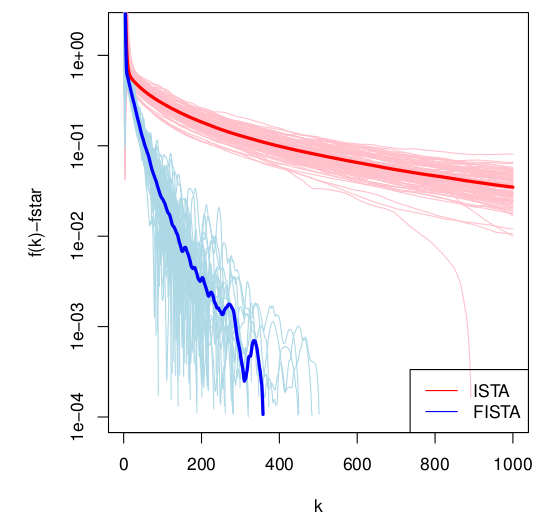
\includegraphics[width=0.5\textwidth]{scribe1.png}
\caption{Performance of ISTA vs FISTA for Lasso Regression (n=100,p=500)}
\end{figure}

\begin{figure}[ht!]
\centering
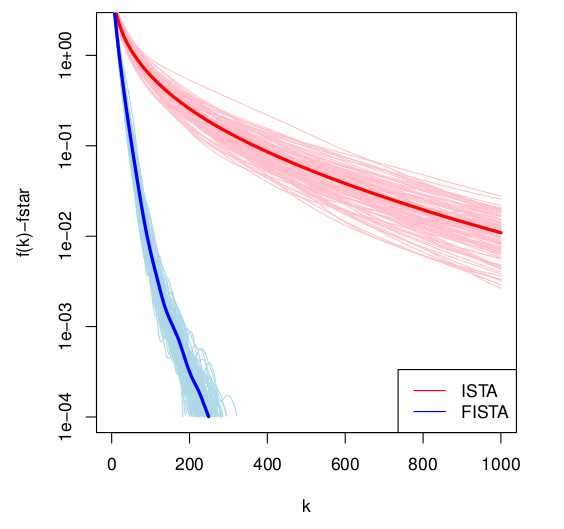
\includegraphics[width=0.5\textwidth]{scribe2.png}
\caption{Performance of ISTA vs FISTA for Lasso Logistic Regression (n=100,p=500)}
\end{figure}

\pagebreak

\section{Failure Cases for Acceleration}
Acceleration achieves the optimal $O(1/k^2)$ convergence rate for gradient based methods. However, it does not do so under all conditions. In some cases it might perform similar to non-accelerated methods and in some others it might actually hurt performance. Some cases are presented wherein acceleration fails to do well. 

\subsection{Warm Starts}
In iterative algorithms warm starting can be an effective strategy to speed up convergence. For e.g. in cross validation runs for Lasso , one can use the optimal $\hat{x}$ found in the previous iteration as a warm start for the next iteration. Let the tuning parameters for lasso be 
\[
\lambda_1 \geq \lambda_2 \geq \dotsc \geq \lambda_r
\]
When solving for $\lambda_1$, initialize $x^{(0)} = 0$ and record solution $\hat{x}(\lambda_1)$. Now, reuse this value such that when solving for $\lambda_j$, initialize $x^{(0)}(\lambda_j) = \hat{x}(\lambda_{j-1})$. It has been observed that over a fine grid of values, generalized gradient descent can perform just as well as accelerated version when using warm starts.

\subsection{Matrix Completion}
In the case of matrix completion, acceleration and even backtracking can hurt performance. The matrix completion problem is described in Lecture 8. Briefly, Given a matrix A, only some entries $(i,j) \in \Omega$ of which are visible to you, you want to   fill in the rest of entries, while keeping the matrix low rank. We solve, 
\[
\min_{X}\frac{1}{2}\lVert P_\Omega(A) - P_\Omega(X) \rVert_F^2 + \lambda\lVert X \rVert_*
\]
 where $\lVert X \rVert_* = \sum_{i=1}^r \sigma_i(X)$ is the nuclear norm, r is the rank of X and $P_\Omega(\cdot)$ is the projection operator,
 \[
 \left[P_\Omega(X) \right]_{ij} = \begin{cases}
 X_{ij} &\quad (i,j) \in \Omega \\
 0 &\quad (i,j) \notin \Omega
 \end{cases}
 \]
the gradient descent updates, also known as the \emph{soft-impute} algorithm are 
\[
X^+ = S_\lambda(P_\Omega(A) + P_\Omega^\perp(X))
\]
where $S_\lambda(\cdot)$ is the matrix soft-thresholding operator which requires the SVD to compute as $S_\lambda(X) = U\Sigma_\lambda V^T$ where $(\Sigma_\lambda)_{ii}=\max\{\Sigma_{ii}-\lambda,0\}$ . Calculating the SVD can be expensive and can cost upto $O(mn^2)$ operations. 


This can be expensive for the backtracking search method since each backtracking loop evaluates the generalized $G_t(X)$ at various values of t and this involves solving the prox function. This equates to calling the SVD several times and can be slow. 


The matrix completion problem does not work well with acceleration as well, since acceleration involves changing the argument passed to the prox function. We pass $y-t\nabla g(y)$ instead of $x - t\nabla g(x)$. This can make the matrix high rank which makes the computation of SVD more expensive. 


Here is an example where using acceleration performs worse than soft-impute~\cite{M11}. 

\begin{figure}[ht!]
\centering
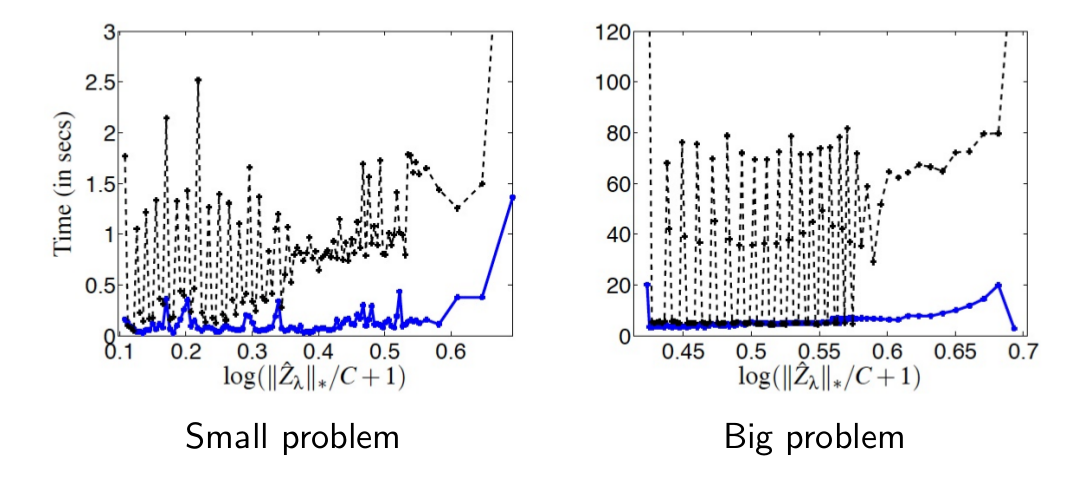
\includegraphics[width=0.9\textwidth]{scribe3.png}
\caption{Performance of Soft impute vs Accelerated grad descent on a small and a big problem}
\end{figure}

\pagebreak

\section*{References}
\beginrefs
\bibentry{M11}{\sc R.~Mazumder} and {\sc T.~Hastie} and {\sc R.~Tibshirani}
``Spectral Regularization Algorithms for Learning Large Incomplete Matrices,''
{\it The Journal of Machine Learning Research},
2011, pp.~2287--2322.
\endrefs

% **** THIS ENDS THE EXAMPLES. DON'T DELETE THE FOLLOWING LINE:

\end{document}





